
% This LaTeX was auto-generated from MATLAB code.
% To make changes, update the MATLAB code and republish this document.

\documentclass{article}
\usepackage{graphicx}
\usepackage{color}
\usepackage{graphicx}

\sloppy
\definecolor{lightgray}{gray}{0.5}
\setlength{\parindent}{0pt}

\begin{document}

    
    
\subsection*{Contents}

\begin{itemize}
\setlength{\itemsep}{-1ex}
   \item AMSC 460 - HW11
   \item Problem 1
   \item Problem 2 
\end{itemize}


\subsection*{AMSC 460 - HW11}

\begin{verbatim}
clear all; format compact; close all; syms f(x) x y z
\end{verbatim}


\subsection*{Problem 1}

\begin{par}
   Find a quartic Hermite polynomial that interpolates
   \[p(0)=1,\quad p'(0)=-1,\quad p(1)=-2,\quad p'(1)=2,\quad p(2)=2.\]
\end{par} \vspace{1em}
\begin{par}
\[L_0(x) = \frac{(x-x_1)(x-x_2)}{(x_0-x_1)(x_0-x_2)} =  \frac{(x-1)(x-2)}{(-1)(-2)} = \frac{1}{2}(x^2-3x+2)\]
\begin{par}
   now differentiate the equation above 
   \[L_0'(x) = (1/2)(x^2-3x+2)*\frac{d}{dx}\ = \frac{1}{2}*(2x-3) \]
\end{par} \vspace{1em}
\begin{par}
   \[L_1(x) = \frac{(x-x_0)(x-x_2)}{(x_1-x_0)(x_1-x_0)} =  \frac{(x-0)(x-2)}{(1)(-1)} =-x^2+2x\]
\begin{par}
   now differentiate the equation above 
   \[L_1'(x) = = -2x-2 \]
\end{par} \vspace{1em}
\end{par} \vspace{1em}
\begin{par}
   similarly, we can have \[L_2(x) =\frac{1}{2}(x^2-2) \] 
   \[L_2'(x) =\frac{1}{2}(2x-1) \] 
   \[L_2(x_2) =\frac{1}{2}(2*2-1) = \frac{3}{2} \] 
\end{par} \vspace{1em}

\begin{par}
   Now \[p4(x) =  f[0]+f_[0,0,1](x^2)+f[0,0,1,1](x^2)(x-1) + f[0,0,1,1,2]x^2(x-1)^2\]
   \[ = -10x^4+27x^3-19x^2-x+1\]
\end{par} \vspace{1em}


\end{par} \vspace{1em}


\subsection*{Problem 2 (}

\begin{par}Consider the function 
	\[f(x) = \frac{e^{3x}\sin(200x^2)}{1+20x^2}\]
on the interval $0\le x\le 1$. The goal of this problem is to observe the error reduction in cubic spline interpolation when increasing the number of nodes.
\end{par} \vspace{1em}
\begin{par}
(a)Show that $|J(x)|\le 1$, $|J'(x)|\le 1$, $|J''(x)|\le 1$, and in general that $|J^{(k)}(x)|\le 1$ for any positive integer $k$.
\end{par} \vspace{1em}

\begin{verbatim}
syms x n
f(x) = (exp(3*x)*sin(200*x^2)/(1+20*x^2))
ezplot(f(x))
\end{verbatim}

        \color{lightgray} \begin{verbatim}f(x) =
(exp(3*x)*sin(200*x^2))/(20*x^2 + 1)
\end{verbatim} \color{black}   

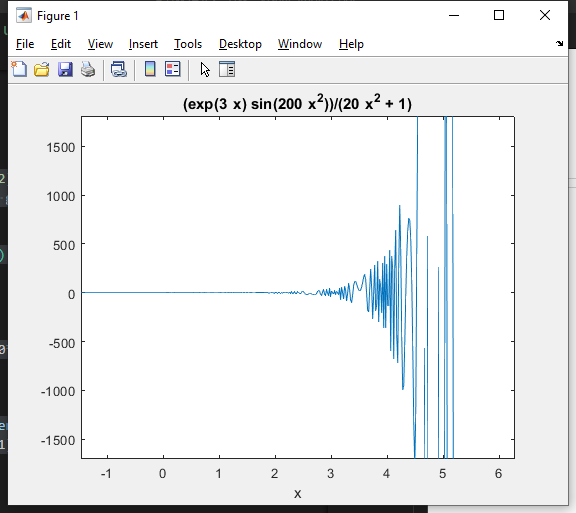
\includegraphics{sd.png}

\begin{par}
   (b)Write a short script using the MATLAB \texttt{spline} command, that interpolates $f(x)$ at equidistant points $x_i = i/n$ ($i=0,1,...,n$), where $n$ is an arbitary fixed number of subintervals prescribed by the user.
\end{par} \vspace{1em}
\begin{verbatim}
   z=6
   test = 1: z
   for k =1:z
       i = 0:test(k)
       xi = i/z
       spline(xi,fx)
   end
\end{verbatim}

\color{lightgray} \begin{verbatim}z =
6
test =
1     2     3     4     5     6
i =
0     1
xi =
 0    0.1667
\end{verbatim} \color{black}

\begin{par}
(c)For $n=2^j$, $j=4,5,...,14$, run your script and record the maximum value of the error $e(x) := |f(x)-s(x)|$ at the points \texttt{x=0:0.001:1}, where $s(x)$ denotes the cubic spline interpolant. In other words, for each $n$, compute $\max_{x\in 0:0.001:1}e(x)$ and store this value. (For efficient coding, you shouldn't loop through all $x$. Vectorize $f$ and use the \texttt{max} command to compute $\max_{x\in 0:0.001:1}|f(x)-s(x)|$ in one shot.) 
\end{par} \vspace{1em}

\begin{par}
This is asking for the each n max||f(x)- s(x)||
\end{par} \vspace{1em}


\begin{par}
   (d)Plot the errors against n on a loglog plot and make observations
\end{par} \vspace{1em}


\end{document}

